\documentclass[problem]{mcs}

\begin{pcomments}
  \pcomment{PS_top_sort_for_closure_of_DAG}
  \pcomment{from: S09.ps6, S08.ps6, S06.ps4 (adapted)}
  \pcomment{revised by ARM, 2/28/10}
\end{pcomments}

\pkeywords{
  digraphs
  DAGs
  topological_sort
  transitive_closure
  paths
}

%%%%%%%%%%%%%%%%%%%%%%%%%%%%%%%%%%%%%%%%%%%%%%%%%%%%%%%%%%%%%%%%%%%%%
% Problem starts here
%%%%%%%%%%%%%%%%%%%%%%%%%%%%%%%%%%%%%%%%%%%%%%%%%%%%%%%%%%%%%%%%%%%%%

\begin{problem}
The following procedure can be applied to any digraph, $G$:

\begin{enumerate}

\item\label{del-cycle} Delete an edge that is traversed by a directed cycle.

\item\label{del-uncover} Delete edge $\diredge{u}{v}$ if there is a
  directed path from vertex $u$ to vertex $v$ that does not traverse
  $\diredge{u}{v}$.

\item\label{add-edge} Add edge $\diredge{u}{v}$ if there is no directed
  path in either direction between vertex $u$ and vertex $v$.

\end{enumerate}
  Repeat these operations until none of them are applicable.

This procedure can be modeled as a state machine.  The start state is
$G$, and the states are all possible digraphs with the same vertices as
$G$.

\bparts

\ppart\label{G1234} Let $G$ be the graph with vertices $\set{1,2,3,4}$ and edges
\[
\set{\diredge{1}{2}, \diredge{2}{3}, \diredge{3}{4}, \diredge{3}{2}, \diredge{1}{4}}
\]
What are the possible final states reachable from $G$?

\begin{solution}
There are six::
\begin{align*}
\set{\diredge{1}{2}, \diredge{2}{3}, \diredge{3}{4}}\\
\set{\diredge{1}{3}, \diredge{3}{2}, \diredge{2}{4}}\\
\set{\diredge{3}{1}, \diredge{1}{2}, \diredge{2}{4}}\\
\set{\diredge{1}{3}, \diredge{3}{4}, \diredge{4}{2}}\\
\set{\diredge{3}{1}, \diredge{1}{4}, \diredge{4}{2}}\\
\set{\diredge{3}{4}, \diredge{4}{1}, \diredge{1}{2}}\\
\end{align*}

The last five can all be reached by deleting first $\diredge{1}{4}$ and
then $\diredge{2}{3}$.

\end{solution}
\eparts

A \emph{line graph} is a graph whose edges can all be traversed by a
directed simple path.  All the final graphs in part~\eqref{G1234} are
line graphs.

\iffalse

For example, the two-ended graph below is a line graph of
length 4.
\begin{figure}[h]\redrawn
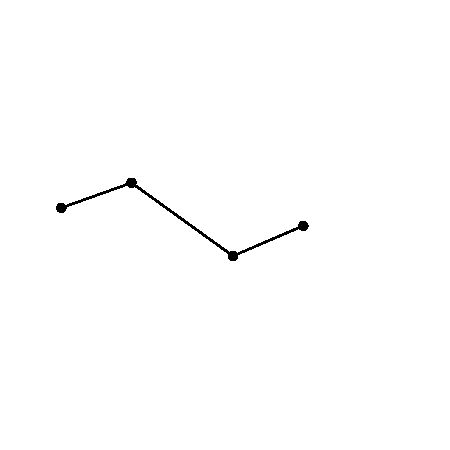
\includegraphics{ps4-path}
\end{figure}
\fi

\bparts

\ppart\label{lineg} Prove that if the procedure terminates with a
digraph, $H$, then $H$ is a line graph with the same vertices as $G$.

\hint Show that if $H$ is \emph{not} a line graph, then some operation
must be applicable.

\begin{solution}
  Since vertices are not changed in any transition, $H$ will have the
  same vertices as $G$.  So we need only show that if $H$ is
  \emph{not} a line graph, then an operation is applicable.

  Now if $H$ has a directed cycle, then operation~\ref{del-cycle}.\
  applies.  So $H$ must be a DAG.  Further, if there are two
  incomparable elements, $u \neq v$ in the partial order defined by
  this DAG, then operation~\ref{add-edge}.\ would be applicable to add
  either $\diredge{u}{v}$ or $\diredge{u}{v}$.  So the DAG must
  define a total order.
  
  All that remains is to prove that no vertex has in-degree or
  out-degree greater than one.  The proof for in-degree and out-degree
  is virtually the same, and we'll just prove that out-degree is at
  most one.

  So suppose to the contrary that in $H$, a vertex $u$ has out-degree
  of 2 or more.  So there are vertices $v \neq w$ and edges
  $\diredge{u}{v}$ and $\diredge{u}{w}$ in $H$.  Now since $H$ defines
  a total order, there must be a directed simple path, $\pi$, in one
  direction or the other between $v$ and $w$; moreover $\pi$ does not
  go through $u$ (if it did, there would be a cycle).  Hence, the path
  $u,\pi$ goes from $u$ to $w$ without traversing $\diredge{u}{w}$,
  which means that $\diredge{u}{w}$ could be deleted by applying
  operation~\ref{del-uncover}.
\end{solution}

\ppart\label{DAG-invar} Prove that being a DAG is a preserved
invariant of the procedure.

\begin{solution}
  Deleting an edge cannot create a cycle, and neither can adding
  an edge between unconnected vertices.  So if there was no cycle in a graph,
  there wouldn't be any after one state transition.
\end{solution}

\ppart\label{top-sort} Prove that if $G$ is a DAG and the procedure
terminates, then the path relation of the final line graph is a
topological sort of $G$.

\hint Verify that the predicate
\[
P(u,v)\eqdef \text{there is a directed path from $u$ to $v$}
\]
is a preserved invariant of the procedure, for any two vertices $u,v$ of a DAG.

\begin{solution}
\begin{proof}
  To prove $P(u,v)$ is an invariant, suppose $P(u,v)$ holds in some
  DAG $H$.  Then operation~\ref{del-cycle}.\ won't be applicable since
  there are no cycles. Also, since adding an edge preserves all
  existing paths, operation~\ref{add-edge}.\ will preserve $P(u,v)$.
  This leaves only operation~\ref{del-uncover},\ to consider.

  So suppose operation~\ref{del-uncover}.\ is applied to delete an edge
  $\diredge{x}{y}$ of $H$.  By definition of the operation, this would
  only be possible if there remains a directed path, $\pi$, from $x$
  to $y$.  Hence for any directed path that traversed
  $\diredge{x}{y}$, there remains a directed path between the same
  endpoints obtained by replacing edge $\diredge{x}{y}$ by $\pi$.  So
  $P(u,v)$ will still hold.

  Since $G$ is a DAG, its path relation is a partial order, $\preceq_G$.  
  By part~\eqref{lineg}, the procedure terminates with a DAG, $H$, that
  defines a total order, $\preceq_H$.  So to show that $\preceq_H$ is a topological sort of 
  $\preceq_G$, we need only check that
  \[
  u \preceq_G v \QIMPLIES u \preceq_H v.
  \]
  But $u \preceq_G v$ is equivalent to $P(u,v)$ holding in $G$, and
  since $P$ is preserved, $P(u,v)$ still holds in $H$, and this is
  equivalent to $u \preceq_H v$.

\end{proof}
\end{solution}

\ppart Prove that if $G$ is finite, then the procedure terminates.

\hint Let $s$ be the number of simple cycles, $e$ be the number of
edges, and $p$ be the number of pairs of vertices with a directed path
(in either direction) between them.  Note that $p \leq n^2$ where $n$
is the number of vertices of $G$.  Find coefficients $a, b,c$ such
that $as+ bp + e +c$ is a strictly decreasing, $\naturals$-valued
variable.

\begin{solution}

Since $s,e \in \naturals$ and $0 \leq p \leq n^2$, where $n$ is the
number of vertices of $G$, the value
\[
2n^2s - 2p + e + 2n^2
\]
is always nonnegative.  We claim it is strictly decreasing.  To prove
this, we consider the effect of the three kinds of operations.

Adding edge $\diredge{u}{v}$ by operation~\ref{add-edge}.\ adds one to
$e$ and leaves $s$ unchanged.  Also, pairs of vertices connected by a
directed path remain connected after adding an edge, and adding
$\diredge{u}{v}$ creates the new connected pair, $(u,v)$, so $p$
increases by at least one.  Therefore $2n^2s-2p+e$ decreases by at
least one.

Deleting an edge by operation~\ref{del-cycle}.\ decreases $e$ and $s$ by
at least one.  It could also decrease $p$, but not by more than the
total number, $n^2$, of pairs of vertices, so $2n^2s-2p+e$ decreases by
at least one.

Finally, deleting an edge decreases $e$ by one and never increases
$s$.  Further, deleting an edge by operation~\ref{del-uncover}.\ does
not change the path relation, as explained in the solution to
part~\eqref{DAG-invar}, so $p$ does not change.  so $2n^2s-2p+e$
decreases by at least one.

\end{solution}
\eparts

\end{problem}

%%%%%%%%%%%%%%%%%%%%%%%%%%%%%%%%%%%%%%%%%%%%%%%%%%%%%%%%%%%%%%%%%%%%%
% Problem ends here
%%%%%%%%%%%%%%%%%%%%%%%%%%%%%%%%%%%%%%%%%%%%%%%%%%%%%%%%%%%%%%%%%%%%%

\endinput

